\documentclass[a4paper,10pt]{article}

%----------------------------------------------------------------------------------------
%	PACKAGES
%----------------------------------------------------------------------------------------
\usepackage[margin=0.55in]{geometry}
\usepackage{latexsym}
\usepackage{enumitem}
\usepackage{hyperref}
\usepackage{xcolor}
\usepackage{url}
\usepackage{titlesec}
\usepackage{fontawesome5}
\usepackage{array}
\usepackage{tabularx}
\usepackage{graphicx}

\hypersetup{
    pdftitle={SK Saif Ibna Ezhar Arko - Academic CV},
    pdfauthor={SK Saif Ibna Ezhar Arko},
    pdfsubject={Curriculum Vitae},
    colorlinks=true,
    urlcolor=blue!70!black,
    linkcolor=black,
    citecolor=blue!70!black
}

%----------------------------------------------------------------------------------------
%	SECTION FORMATTING
%----------------------------------------------------------------------------------------
\titleformat{\section}
{\large\bfseries\scshape}
{}{0em}
{}
[\vspace{-7pt}\rule{\textwidth}{0.6pt}\vspace{-6pt}]

\titlespacing{\section}{0pt}{7pt}{3pt}

\setlist[itemize]{
    leftmargin=1.2em,
    itemsep=0pt,
    topsep=1pt,
    parsep=0pt
}

\setlength{\parindent}{0pt}
\pagestyle{empty}
\raggedbottom

%----------------------------------------------------------------------------------------
\begin{document}

%----------------------------------------------------------------------------------------
%	HEADER
%----------------------------------------------------------------------------------------
\begin{minipage}[b]{0.68\textwidth}
    \raggedright
    {\Huge \textbf{SK Saif Ibna Ezhar Arko}} \\[3pt]
    {\small 14 Bonogram Road, Wari, Dhaka 1203, Bangladesh} \\[1pt]
    {\small
    \faPhone\ +880 1600 152614 \quad | \quad
    \faEnvelope\ \href{mailto:saifibnaezhararko1@gmail.com}{saifibnaezhararko1@gmail.com} \\[1pt]
    \faLinkedin\ \href{https://www.linkedin.com/in/sk-saif-ibna-ezhar-arko-0140aa203}{LinkedIn} \quad | \quad
    \faGithub\ \href{https://github.com/saifibnaezhararko}{GitHub} \quad | \quad
    \faGlobe\ \href{https://saifibnaezhararko.github.io/}{Portfolio}
    }
\end{minipage}\hfill
\begin{minipage}[b]{0.28\textwidth}
    \raggedleft
    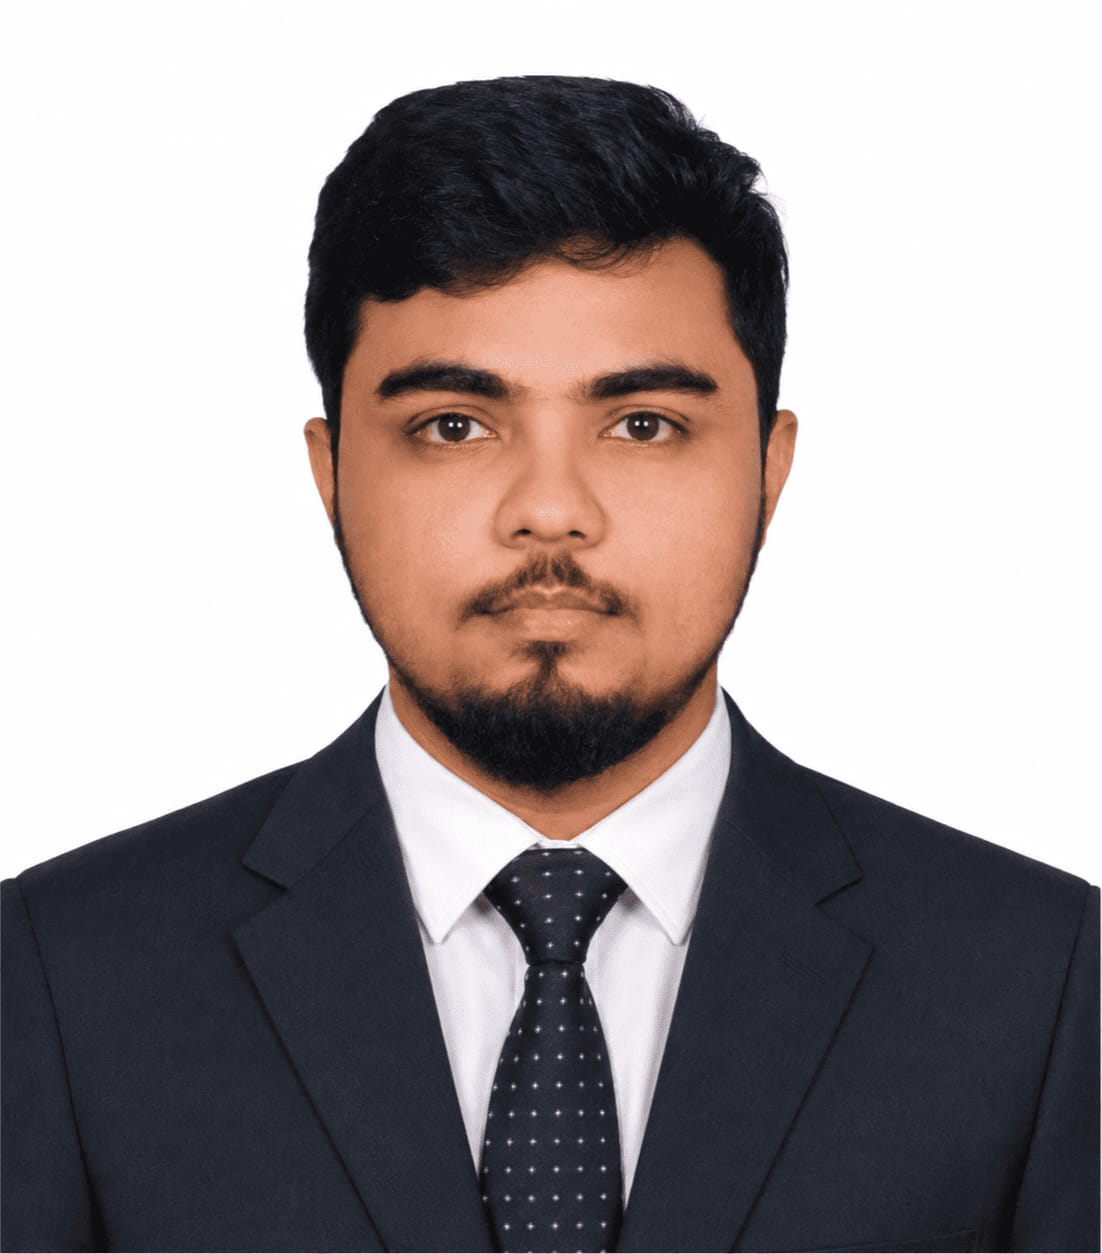
\includegraphics[width=2.9cm, height=2.9cm, keepaspectratio]{photo.jpeg}
\end{minipage}

\vspace{4pt}

%----------------------------------------------------------------------------------------
%	RESEARCH INTERESTS
%----------------------------------------------------------------------------------------
\section*{Research Interests}

Quantum Information Theory \textbullet{}
Quantum Computing and Algorithms \textbullet{}
Quantum Cryptography \textbullet{}
Quantum Machine Learning \textbullet{}
Adversarial Robustness of Quantum Models \textbullet{}
Post-Quantum Cryptography.

%----------------------------------------------------------------------------------------
%	EDUCATION
%----------------------------------------------------------------------------------------
\section*{Education}

\textbf{BRAC University}, Dhaka, Bangladesh
\hfill
\textit{2026}
\\
\textit{B.Sc.\ in Computer Science and Engineering} --- CGPA: \textbf{3.20 / 4.00}

\begin{itemize}
    \item \textbf{Undergraduate Thesis:}
    \textit{Quantum-Aware Image Encoding and Adversarial Perturbation}

    \item \textbf{Relevant Coursework:}
    Quantum Computing, Quantum Error Correction, Quantum Algorithms, Machine Learning,
    Pattern Recognition, Data Structures \& Algorithms, Linear Algebra, Probability \& Statistics.
\end{itemize}

\vspace{2pt}
\textbf{Notre Dame College}, Dhaka
\hfill
\textit{2020}
\\
\textit{Higher Secondary Certificate (Science)} --- GPA: \textbf{5.00 / 5.00}

\vspace{2pt}
\textbf{St.\ Gregory's High School and College}, Dhaka
\hfill
\textit{2018}
\\
\textit{Secondary School Certificate (Science)} --- GPA: \textbf{5.00 / 5.00}

%----------------------------------------------------------------------------------------
%	RESEARCH EXPERIENCE
%----------------------------------------------------------------------------------------
\section*{Research Experience}

\textbf{Undergraduate Thesis Researcher} --- BRAC University, Dept.\ of CSE
\hfill
\textit{2024 -- Present}
\\
\textit{Supervisor: Ipshita Bonhi Upoma, Lecturer, Department of CSE, BRAC University}

\begin{itemize}
    \item Developing theoretical frameworks for encoding classical image data into quantum states via amplitude and basis encoding, and analyzing their robustness against adversarial noise.

    \item Studying trade-offs between encoding fidelity, circuit depth, and resilience to bit-flip and phase-flip channels.
\end{itemize}

\vspace{2pt}
\textbf{Student Researcher} --- ELITE Research Lab LLC
\hfill
\textit{Sept.\ 2026 -- Jan.\ 2027}
\\
\textit{Supervisor: Md Kishor Morol}

\begin{itemize}
    \item Conducting research at the intersection of quantum computing and machine learning in collaboration with industry experts.
\end{itemize}

\vspace{2pt}
\textbf{Research Intern, QIntern 2026 Global Internship} --- QWorld
\hfill
\textit{Summer 2026}
\\
\textit{Supervisor: Dr.\ Maha A. Metawei}

\begin{itemize}
    \item Project: \textit{Accelerating hybrid quantum-classical machine learning tasks on HPC platforms (QNLP)}.

    \item Implemented high-performance quantum circuit simulations and tensor network optimizations to scale hybrid algorithms on distributed clusters; extended core framework classes (\textit{Ansatz}, \textit{Reader}) and built unified data format conversion scripts.
\end{itemize}

\vspace{2pt}
\textbf{Research Intern, QIntern 2025 Global Internship} --- QWorld
\hfill
\textit{Summer 2025}
\\
\textit{Supervisors: Dr.\ Kumar Prateek, Dr.\ Soumyadev Maity}

\begin{itemize}
    \item Project: \textit{Design of Quantum-Anamorphic Encryption Against Coercive Surveillance}.
    Prototyped anamorphic quantum encryption schemes providing deniability against coercive adversaries.

    \item \textbf{Awarded 3rd Best Project globally} among submissions worldwide; collaborated with an international team across multiple countries.
\end{itemize}

%----------------------------------------------------------------------------------------
%	PROFESSIONAL EXPERIENCE
%----------------------------------------------------------------------------------------
\section*{Professional Experience}

\textbf{Datasoft Systems Bangladesh Limited}, Dhaka
\hfill
\textit{December 2025 -- Present}
\\
\textit{Software Developer (AI and Quantum Department)}

\begin{itemize}
    \item Deploy and operate self-hosted LLM inference infrastructure with \texttt{llama.cpp} and \texttt{llama-server}, serving a 228B-parameter (10B active) Mixture-of-Experts model in quantized GGUF format across heterogeneous single-GPU nodes.

    \item Designed the \textit{Hermes Agent} framework: model-switching, multi-provider LLM routing (NVIDIA NIM, DeepSeek, OpenRouter, local Ollama) behind an authenticated API gateway running as a supervised \texttt{systemd} service.

    \item Built LangGraph-based agentic SQA workflows executing multi-step verification across Django/React/PostgreSQL projects, and delivered \textit{iSAGE}, an internal assistant UI over the local LLM backend.

    \item Engineer production Python systems for document processing and workflow automation, including distributed scraping and ETL pipelines; contributed to the terminal operating system of Chittagong Sea Port.
\end{itemize}

\vspace{2pt}
\begin{minipage}{\textwidth}
\textbf{Maxcode Lab}, Dhaka --- \textit{Python Developer Intern}
\hfill
\textit{October 2025 -- December 2025}

\begin{itemize}
    \item Engineered Python tools for web scraping, automation, database management, and REST API integration.
\end{itemize}
\end{minipage}

%----------------------------------------------------------------------------------------
%	SELECTED PROJECTS
%----------------------------------------------------------------------------------------
\section*{Selected Projects}

\textbf{QVTM --- Quantum Variable Topic Model} (Global Quantum Hackathon 2024)
\hfill
\href{https://github.com/saifibnaezhararko/QVTM}{[GitHub]}

\begin{itemize}
    \item Built an encoder--decoder variational quantum model using \textbf{amplitude embedding} to represent text in Hilbert space, optimized with a composite \textbf{KL-divergence}, \textbf{Cross-Entropy}, and \textbf{MMD} objective.

    \item Achieved a \textbf{Topic Diversity score of 1.0} with improved coherence over Latent Dirichlet Allocation baselines.
\end{itemize}

\textbf{Monkeypox Classification Using a Hybrid Quantum CNN (HQCNN)}
\hfill
\href{https://tinyurl.com/3kvmhea8}{[GitHub]}

\begin{itemize}
    \item Combined classical feature extraction with parameterized quantum circuits and benchmarked against purely classical CNN and EfficientNetB3 transfer-learning baselines for medical image diagnosis.
\end{itemize}

\textbf{Lexora --- Bengali-First English Vocabulary Learning Platform}
\hfill
\href{https://lexora-sipb.onrender.com/}{[Live]}
\href{https://github.com/saifibnaezhararko/Lexora-English-Vocabulary-Learning-App-Django}{[GitHub]}

\begin{itemize}
    \item Built a Django 5 and HTMX progressive web app (\textasciitilde 9,900 lines of Python across five apps, 89 tests) for GRE and IELTS preparation, serving 1{,}468 words in 62 sequential packs with paired Bangla and English meanings.

    \item Implemented a full \textbf{SuperMemo-2} spaced-repetition scheduler alongside a Leitner five-box ladder and an \textbf{Ebbinghaus retention-curve} exam forecast, plus study modes spanning timed drills, dictation, confusable-pair training, and an AI-driven debate arena.
\end{itemize}

\textbf{NLP Similarity Classifier --- Bidirectional LSTM Siamese Network}
\hfill
\href{https://github.com/saifibnaezhararko/NLP-Similarity-Classifier-Bidirectional-LSTM-based-Siamese-network-with-multiple-merge-strategies}{[GitHub]}

\begin{itemize}
    \item Designed a TensorFlow/Keras Siamese network for paraphrase identification, fusing sentence embeddings with Jaccard and fuzzy-matching features across four merge strategies; an augmentation pipeline generated \textbf{7{,}400+ synthetic samples}, evaluated via ROC curves and confusion matrices.
\end{itemize}

\textbf{Other projects:}
\href{https://tinyurl.com/59uzaj9r}{Stock price forecasting --- ARIMA vs.\ LSTM};
\href{https://github.com/saifibnaezhararko/SmartCare-Healthcare-Based-Django-website-}{SmartCare}, a Django healthcare management platform;
\href{https://github.com/saifibnaezhararko/CSE423_Lab-Project-3D-Ball-Roller}{3D Ball Roller}, a physics-based OpenGL game in Python.

%----------------------------------------------------------------------------------------
%	COMMUNITY, TEACHING & SERVICE
%----------------------------------------------------------------------------------------
\section*{Community Contributions, Teaching, and Professional Service}

\textbf{IBM Qiskit Advocate} (\#129943) --- IBM Quantum
\hfill
\textit{2025 -- Present}

\begin{itemize}
    \item Recognized for sustained contributions to the global quantum community; lead workshops, mentor early-career researchers on Qiskit projects, create tutorials and learning resources, support the community on official Discord and GitHub channels, and organize outreach events and hackathons.
\end{itemize}

\vspace{2pt}
\textbf{QBangladesh --- National Hub of QWorld}, Bangladesh
\hfill
\textit{April 2025 -- Present}
\\
\textit{Founder, Coordinator, and Mentor}

\begin{itemize}
    \item Established and lead the first national quantum computing community in Bangladesh under the QWorld umbrella, building a sustainable ecosystem for quantum education and research.

    \item Deliver hands-on workshops on quantum computing with Python, Qiskit, and Cirq for students nationwide, and mentor early-career researchers on quantum algorithms and simulation.
\end{itemize}

\vspace{2pt}
\textbf{Caretutors Technology Limited}, Dhaka --- \textit{Verified Tutor}
\hfill
\textit{December 2024 -- Present}

\begin{itemize}
    \item Deliver Python instruction covering programming logic, data structures, and core language concepts through personalized, project-based learning plans.
\end{itemize}

%----------------------------------------------------------------------------------------
%	TECHNICAL SKILLS
%----------------------------------------------------------------------------------------
\section*{Technical Skills}

\begin{tabularx}{\textwidth}{@{}lX@{}}
\textbf{Programming:} & Python, C, C++, SQL \\
\textbf{Quantum:} & Qiskit, Cirq, PennyLane (basic), Stim \\
\textbf{ML / DL:} & TensorFlow, Keras, scikit-learn, NumPy, Pandas, Matplotlib, LangGraph \\
\textbf{Web \& Tools:} & Django, HTMX, PostgreSQL, HTML/CSS, OpenGL, Git, Linux, Jupyter, LaTeX \\
\textbf{Languages:} & Bengali (Native), English (Full Professional Proficiency) \\
\end{tabularx}

%----------------------------------------------------------------------------------------
%	HONORS, AWARDS & CERTIFICATIONS
%----------------------------------------------------------------------------------------
\section*{Honors, Awards, and Certifications}

\textbf{Awards:}
3rd Best Project Globally, QIntern 2025 (QWorld);
Diploma in Quantum Anamorphic Encryption, QWorld 2025.

\vspace{2pt}

\textbf{Certifications:}
ICTP Physics Without Frontiers: Bangladesh School on Mathematics for Physics 1 --- Operators on Hilbert Spaces (ICTP, 2026);
Quantum AI Lab --- Quantum Cryptography (Bibliotheca Alexandrina, 2026);
Quantum Business Foundations (IBM, 2026);
Basics of Quantum Information (IBM, 2026);
Pan-African Quantum Challenge 2025 (Africa Quantum Consortium, 2026);
Quantum Random Number Generation (Quantum Security Defence, 2026);
Introduction to Quantum Computing (Qubit by Qubit, 2025);
QCOURSE 501-2: Elements of Quantum Computing and Programming (QWorld, 2025);
QSilver26 and QBronze144 Workshops (QWorld, 2024);
Quantum Machine Learning Fundamentals (Ingenii, 2024).

%----------------------------------------------------------------------------------------
%	REFERENCES
%----------------------------------------------------------------------------------------
\section*{References}

\begin{minipage}[t]{0.48\textwidth}
\textbf{Ipshita Bonhi Upoma} \\
Lecturer, Dept.\ of CSE, School of Data and Sciences \\
BRAC University, Bangladesh \textit{(Thesis Supervisor)} \\
\href{mailto:ipshita.upoma@bracu.ac.bd}{ipshita.upoma@bracu.ac.bd}
\end{minipage}
\hfill
\begin{minipage}[t]{0.48\textwidth}
\textbf{Dr.\ Kumar Prateek} \\
Assistant Professor (Grade-II) \\
Dept.\ of Computer Sc.\ \& Engg., NIT Jalandhar, India \\
\href{mailto:kprateek@nitj.ac.in}{kprateek@nitj.ac.in}
\end{minipage}

\end{document}
